\subsection{The use of locales}

During this project, I had a first contact with the tools that Isabelle uses to manage theories. These are not normally introduced in a basic course on the proof assistant and we had to explore on our own using the existing documentation \cite{ballarin2010tutorial}. We worked both with external locales (such as comm\_group):

\begin{figure}[!htbp]
	\centering
	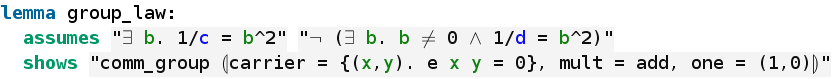
\includegraphics[width=\linewidth,height=\textheight,keepaspectratio]{img/group_law.png}
	\caption{The group law theorem for affine elliptic curves using comm\_group locale}
	\label{fig:grouplaw}
\end{figure}

and our own locales that served to structure and particularize the theories:

\begin{figure}[!htbp]
	\centering
	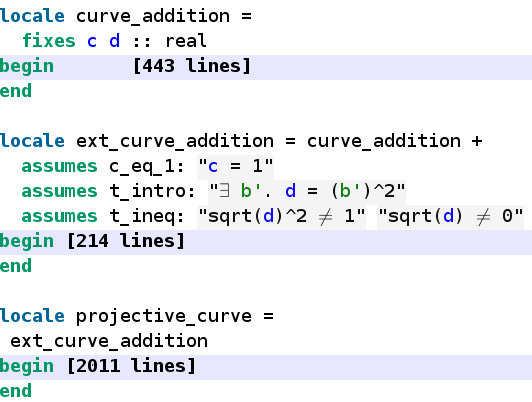
\includegraphics[width=0.8\linewidth,height=0.8\textheight,keepaspectratio]{img/structure.png}
	\caption{General structure of the theory organized in locales}
	\label{fig:grouplaw}
\end{figure}
	
\subsection{The algebra method}

A good understanding of the proving tools at our disposal can save a lot of work. The algebra method \cite{wenzel2019isabelle} has as one of its basic functionalities solving the following quantified formula: 

\begin{align*}
\forall x_1 \ldots x_n. &  \\        
& e_1(x_1,\ldots,x_n) = 0 \land \ldots \land e_m(x_1,\ldots,x_n) = 0 \to \\
& (\exists y_1, \ldots, y_k. \\
& p_{11}(x_1,\ldots,x_n) y_1 + \ldots + p_{1k}(x_1,\ldots,x_n) y_k = 0 \land \\
& \ldots \land \\
& p_{t1}(x_1,\ldots,x_n) y_1 + \ldots + p_{tk}(x_1,\ldots,x_n) y_k = 0) \\
&
\end{align*}

where $e_1,\ldots,e_n$ and $p_{ij}$ are multivariate polynomials in the indicated variables. In our case, $e_i$ could be the hypothesis that we have certain point in the curve and the exists fragment corresponds to the search of division quotients. As a direct consequence, one does not always need to copy the polynomial quotients obtained with Mathematica. Here is an example:

\begin{figure}[!htbp]
	\centering
	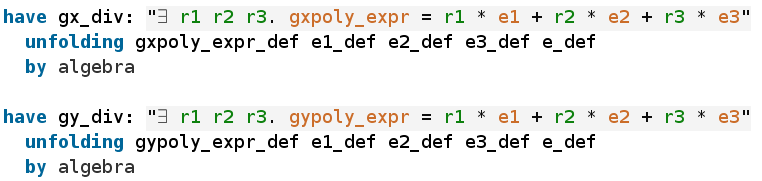
\includegraphics[width=0.8\linewidth,height=0.8\textheight,keepaspectratio]{img/poly_expr.png}
	\caption{Example of polynomial division with the algebra method}
	\label{fig:groebner}
\end{figure}

The variables gxpoly\_expr, gypoly\_expr correspond to given polynomials that are computed explicitly with Mathematica. However, in our case, there is no need to copy the expressions for $r1,r2,r3$ since all we need is their existence. This is in contrast to the situation found in \cite{hales2016group}

\subsection{The use of Gröbner basis}

Hales explicitly uses Gröbner basis to go through the proof of dichotomy. This property is fundamental to establish the well-definition of the group law for projective Edwards curves. To be precise, it would be need in Isabelle whether a given set of polynomials corresponds to a Gröbner basis of a given polynomial ideal. However, the representation of this theory is quite different to ours:

\textit{Essentially, polynomials are represented as ordered lists of monomials, where monomials are represented as pairs consisting of a coefficient and a power-product (I.e., something like $x_0*y_0$); power-products are represented similarly, as ordered lists of indeterminate-exponent-pairs. Indeterminates, finally, are typically represented by natural numbers (although this can be changed easily). See also \cite{maletzky2018grobner}.}

While in practice the computation of Gröbner basis in Isabelle might look like in Figure \ref{fig:groebner}.

\begin{figure}[!htbp]
	\centering
	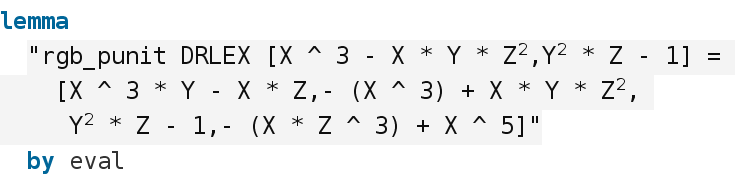
\includegraphics[width=0.8\linewidth,height=0.8\textheight,keepaspectratio]{img/groebner.png}
    \caption{Gröbner basis computation in Reduced\_GB\_Examples.thy}
    \label{fig:groebner}
\end{figure}

more expertise on this theory would be needed in order to connect it with our own. This can be considered as future work since having at our disposal an easy access to verified Gröbner basis computation would have speeded the proof process significantly. 

On the other hand, the algebra method is not capable to solve this problem either. While it computes Gröbner basis for the purpose of proving whether a polynomial is in the generated ideal, this computation is done outside the logic. In particular, it is not proved that the computed basis is indeed a Gröbner basis. 

As a last alternative, one could check by hand that the involved identities hold. This is what Hales suggests in the article when he says: \textit{In particular, our approach does not require the use of Gröbner bases (except in Lemma 4.3.2 where they make an easily avoidable appearance)}. 

Here is one example of such a hand computation. We follow the notation in \cite{hales2016group}. Namely, we focus on equation 19:

$$(x_0^2 - x_1^2,y_0^2 - x_1^2,x_0y_0 - x_1 y_1) \equiv (0,0,0) \; mod \; S_{\pm}$$

where $S_{\pm}$ is the Gröbner basis associated with certain polynomials known to evaluate to zero. One then deduces one by one the corresponding equations:

To start, one deduces the third equality:

$$\delta' = x_0 y_0 \delta_{0x} x_1 y_1 \Big(\frac{1}{t x_0}\Big) \Big(\frac{1}{t y_0}\Big) = 
x_0 y_0 \Big(1 - \frac{t^2 x_1 y_1}{t^2 x_0 y_0}\Big) = x_0y_0 - x_1 y_1$$

Since by assumption $\delta_{-} = 0$ we have the third equality and we note:

$$(1) \; x_0 = x_1 \Big(\frac{y_1}{y_0}\Big)$$

where we have that $x_0,y_0,x_1,y_1 \neq 0$.

For the second, we have:

$$\delta_{+} = t x_0 t_0 \delta_{1x} x_1 y_1 \Big(\frac{1}{tx_0}\Big) \Big(\frac{1}{ty_0}\Big) = t x_0 y_0 \Big(\frac{y_1}{t x_0} - \frac{x_1}{t y_0}\Big) = y_0 y_1 - x_0 x_1 \stackrel{1}{=} y_0 y_1 - x_1^2 \Big(\frac{y_1}{y_0}\Big) = \frac{y_1}{y_0} (y_0^2 - x_1^2)$$

since $\delta',\delta_{+} = 0$, we have the second equation. We also note: 

$$(2) \; \frac{y_1}{y_0} (y_0^2 - x_1^2) = 0$$

Finally, the third equation is obtained as follows:

$$x_0^2 - y_1^2 \stackrel{1}{=} x_1^2 \frac{y_1^2}{y_0^2} - y_1^2 = \Big(\frac{y_1^2}{y_0^2}\Big) (x_1^2 - y_0^2) \stackrel{2}{=} \frac{y_1^2}{y_0^2} (x_1^2 - y_0^2) \stackrel{2}{=} 0$$

One should note that not all the polynomials of $S_{\pm}$ were used in this deduction.

\subsection{The representation of projective elliptic curves}

We have discussed the representation of projective Edwards curves as described in \cite{hales2016group}. The challenge to represent this description is similar to the representation of equivalence classes in \cite{paulson2006defining}. Here is, to start with, the definition of projective addition:

\begin{figure}[!htbp]
	\centering
	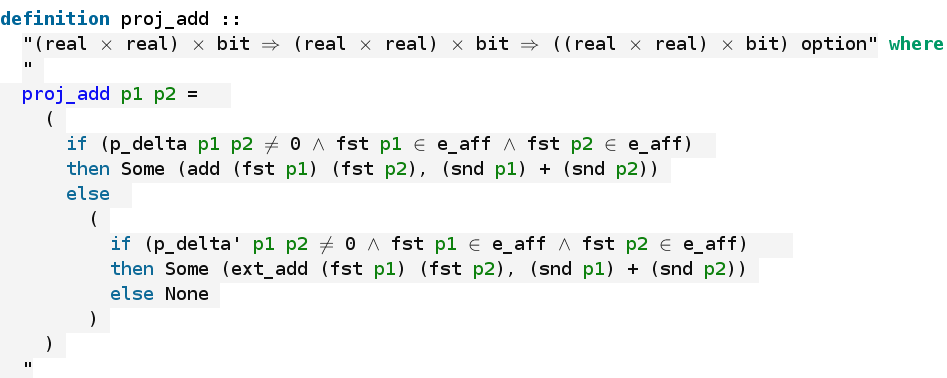
\includegraphics[width=\linewidth,height=\textheight,keepaspectratio]{img/proj_add.png}
	\caption{Projective addition on points}
	\label{fig:proj_add}
\end{figure}

A posteriori, one notes that it would be more convenient to have a more balanced definition without the if-else construct. The version in figure \ref{proj_add_domain} would save some work. For instance, to show that we are in the second branch of the if, we would not need to show that the first branch has a false guard.

\begin{figure}[!htbp]
	\centering
	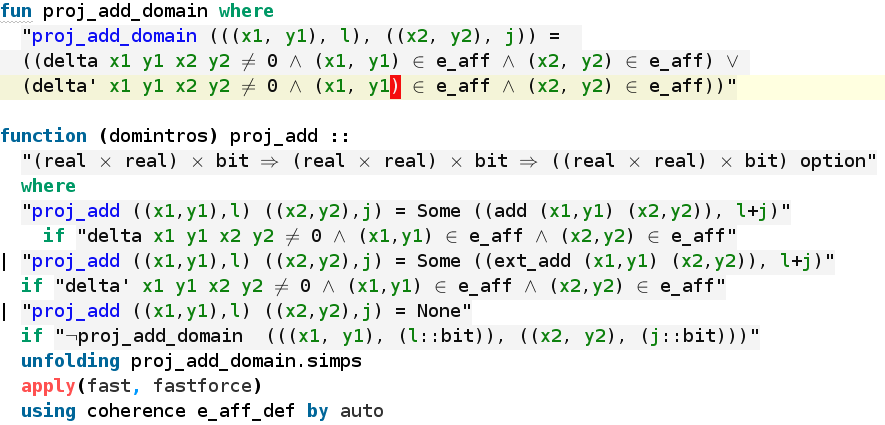
\includegraphics[width=\linewidth,height=\textheight,keepaspectratio]{img/proj_add_domain.png}
	\caption{Balanced version of the projective addition on points}
	\label{fig:proj_add_domain}
\end{figure}

Before introducing proper projective addition, we introduce how are projective points represented:

\begin{figure}[!htbp]
	\centering
	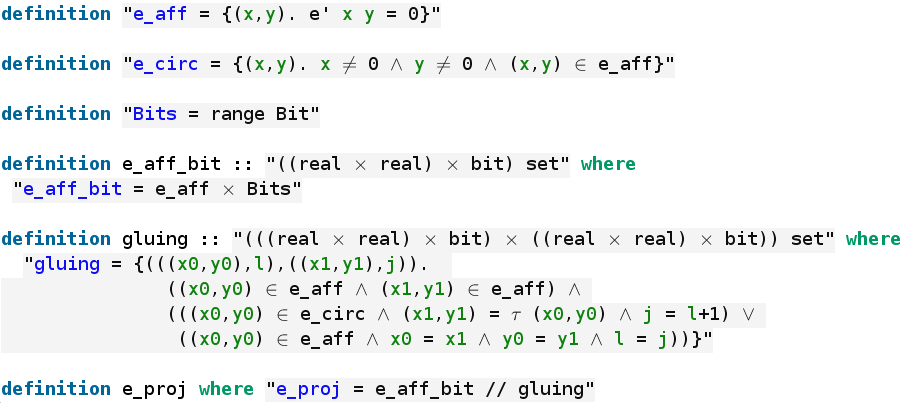
\includegraphics[width=\linewidth,height=\textheight,keepaspectratio]{img/e_proj.png}
	\caption{Projective points representation}
	\label{fig:e_proj}
\end{figure}

So points that satisfy the equation given by $e'$ an which are non-zero are identified with their inversions modulo $\tau$. The other conditions in the equivalence relation only ensure the reflexivity property. It is on these classes of points that projective addition should work. Figure \ref{fig:proj_add_class} shows the adaption of proj\_add to classes. 

proj\_add\_class first selects those pairs that lead to some result, then it actually computes the result and finally identifies equivalent points. Much later, when we prove covering and well-definition we show that indeed the last identification provides only one class. This is the class that is selected with the\_elem in proj\_addition.

\begin{figure}[!h]
	\centering
	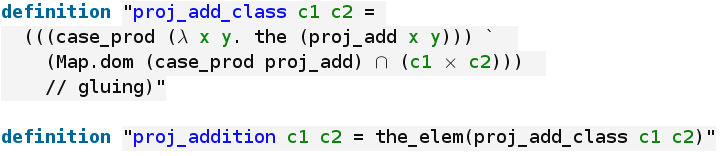
\includegraphics[width=\linewidth,height=\textheight,keepaspectratio]{img/proj_add_class.png}
	\caption{Projective addition on classes of points}
	\label{fig:proj_add_class}
\end{figure}








